If we are to be able to estimate the trajectories based on the initial conditions successfully, we
need to be able to reliably solve the forward problem\footnote{See section \ref{inverse} for a definition
of a forward problem.} for the trajectory of the golf ball. In order
to do this, as stated at the end of the previous chapter, we must find an improved form for $c_D$ which
more accurately describes the physics which occurs during the flight of a ball.

There are a number of approaches to this, and we have attempted a few of them in our investigations
in an attempt to find which of them gives the most reliable results. Any model of golf ball flight which
captures the dynamics of an individual ball will have to use flight data to inform the exact parameters
in a drag function for that ball. Thus, much of this chapter is also concerned with attempting to find 
methods of estimating the parameters for such functions given data on the flight of a particular ball.

This parameter estimation is an example of an inverse problem. Some generalities on such problems are
given in the appendix.

\section{Estimating $c_{D}$ from Experiments} \label{morrison}

As a first attempt at estimating $c_D$, we began by returning to the form given in \citet{Morrison2010}
and discussed in section \ref{sec:drag-crisis}. Recalling that we expect the dimpled surface of the
golf ball to have the affect of moving the point at which the drag crisis occurs to lower Reynolds
numbers, we began by taking Morrison's form for the drag and attempting to change the coefficients to
``move'' the drop in drag to within the range seen within experiments on golf balls.

Here, we attempt to match the function to the experimental data given in various papers which we
have listed before. After some consideration, the following form of $c_D$ can be found to fit
with a number of different experiments

\begin{equation} \label{drag-m-mod}
c_D = \frac{24}{Re} + \frac{2.6(Re/5)}{1 + (Re/5)^{1.52}} + \frac{0.38(Re/121000)^{-7.94}}{1+(Re/121000)^{-8.00}}
+ \frac{Re^{0.83}}{450000} .
\end{equation}

We believe that this form captures the physics we expect to see from the golf ball better than simply
taking a constant value of $c_D$ as in \citet{Robinson2013}. Plotting the original and the modified
form of $c_D$ shows how the drag has moved to within the range we expect to see.
\begin{figure}
% In folder Morrison
\centering
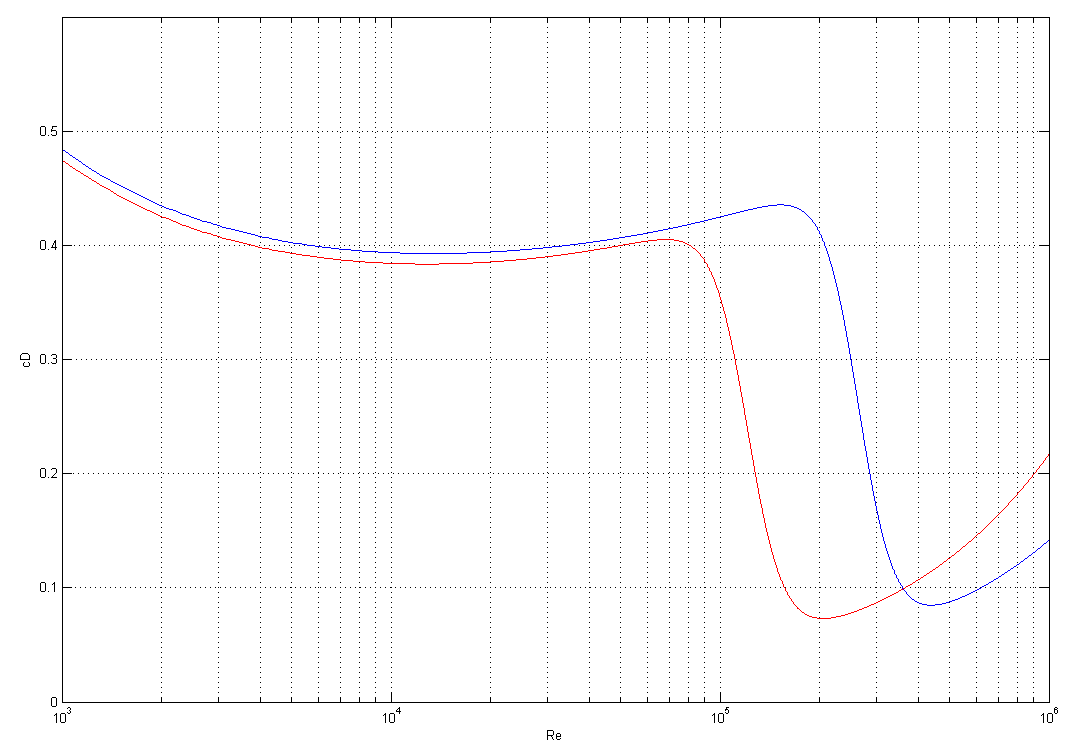
\includegraphics[scale=0.55]{../images/morrison-modified.png}
\caption[Plotting the original Morrison form against a modified version for golf balls]{In blue is the
original $c_D$ function, given in \eqref{drag-m}. In red is the modified form, \eqref{drag-m-mod}, which
takes into account the lower value of Reynolds number where the transition to lower drag occurs.}
\end{figure}

This form has a number of limitations, but does serve to be a good initial start at working out the 
drag for a golf ball. The weaknesses can be summarised as
\begin{itemize}
\item This form of $c_D$ is constant for all types of golf balls, which we know is not the case for
realistic balls, as noted in \citet{Alam2011}.
\item Changing this function for different balls is a matter of hand choosing coefficients in the terms
of \eqref{drag-m-mod}. This method is not at all easy to modify for other balls.
\item While the form of $c_D$ is dimensionless, as we require it to be, there is no dependence on spin
at all, which could be causing significant contributions to the drag.
\end{itemize}

Replacing $c_D$ in the model by Robinson and Robinson by $c_D$ as defined in \eqref{drag-m-mod} does
make a significant change to the resultant trajectory, bringing the height of the ball much closer to
the experimental trajectories and improving the carry of the ball significantly.

% \begin{itemize}
% \item We try to find results for spheres and change them to account for the earlier drag crisis.
% \item Take the function from \citet{Morrison2010} and change the coefficents to ``move'' the drag 
% drop to lower values of $Re$.
% \item This works fairly well but cannot capture all of the behaviour, as other work shows that
% different balls should expect to see different drags \citet{Alam2011}.
% \end{itemize}

\begin{figure}[h]
\centering
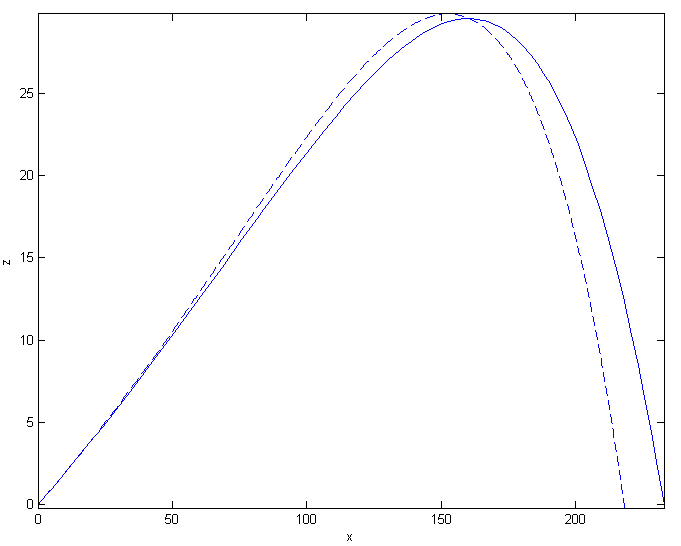
\includegraphics[scale=0.8]{../images/m-mod-data1.png}
\caption[Model with using the modified Morrison form for $c_D$.]{Using the modified Morrison form for $c_{D}$ results 
in a fairly accurate profile. Here the solid line is the model prediction 
and the dashed line is the data.}
\label{m-mod-data1}
\end{figure}

In Figure \ref{m-mod-data1} we see that this form of the drag function brings the model and experimental
results into close agreement with each other. However, viewing the trajectory in 3D reveals that while
the height and carry of the ball are predicted well, the motion along the $y$ axis is not predicted
as well, deviating by approximately $5$m at the end of the trajectory.

\begin{figure}[h]
\centering
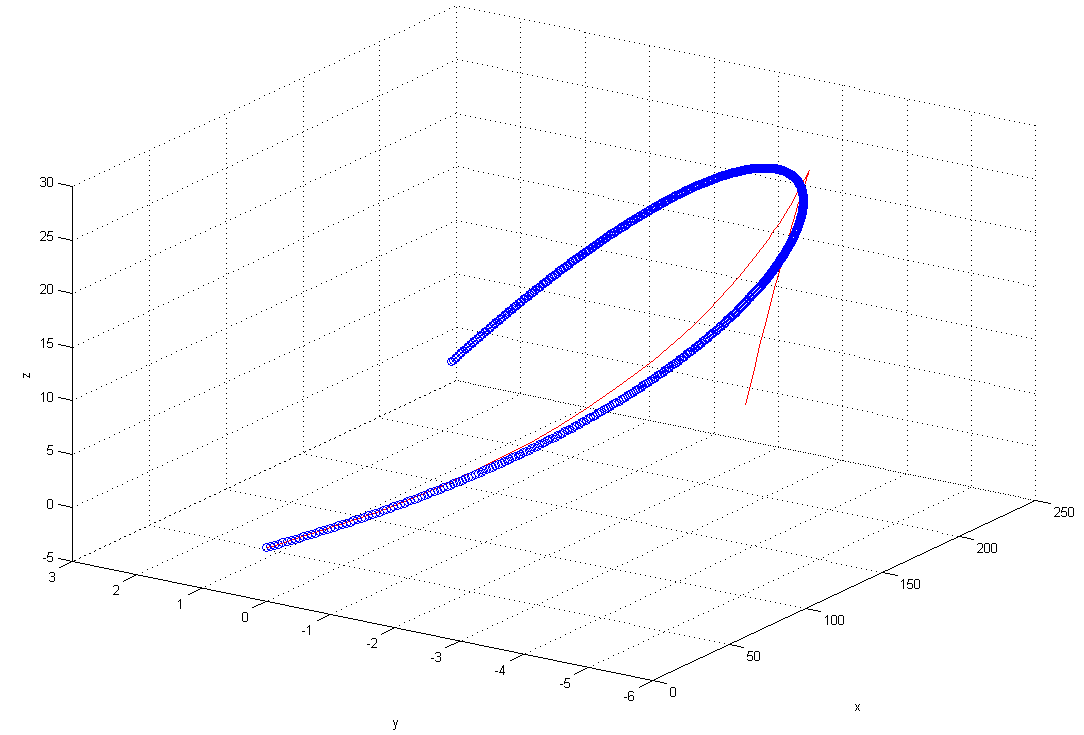
\includegraphics[scale=0.5]{../images/m-mod-data1-3d.png}
\caption[Model with using the modified Morrison form for $c_D$ in 3D.]{This is a 3D plot of Figure \ref{m-mod-data1}.
We note that initially the predicted curve fits the data almost perfectly, being within 1m. Just before
the apex of the curve however the data (plotted with circles) veers back towards the $y=0$ line, whereas
the model (in red) does not have this behaviour.}
\end{figure}

While we see good agreement between the model and the data for this data set, running the model with
a different set of initial conditions and using data taken with a different ball does not yield such
close agreement.

The R\&A provided another data set, this time with 4 trajectories using the same ball. If we select
the second trajectory from this data set to test to test this model against, with the following 
initial conditions
\[
x = -0.112, \,\, y = 0.024, \,\, z = 0, \,\, v_x = 69.438, \,\, v_z = 9.247, \,\, v_y = -0.633, \,\,
|\vec{\omega}| = 370.71,\,\, \theta = \frac{167\pi}{180} .
\]
we find (see Figure \ref{data2-2d}) that the trajectory does not match as closely as the previous data.

This is not that surprising however: the two separate data sets are using different balls, and thus
we would expect the $c_D$ to change between the two balls.

While the modified Morrison form does give better results than simply taking $c_D$ to be constant
it cannot possibly explain how $c_D$ varies for every ball. However, seeing that this form of the drag
brings the model much closer in line with experimental data is encouraging, and implies that factoring
in the drag crisis to the calculation of the model does have a major effect on the resultant trajectories
as we expected it to do so.

\begin{figure}
\centering
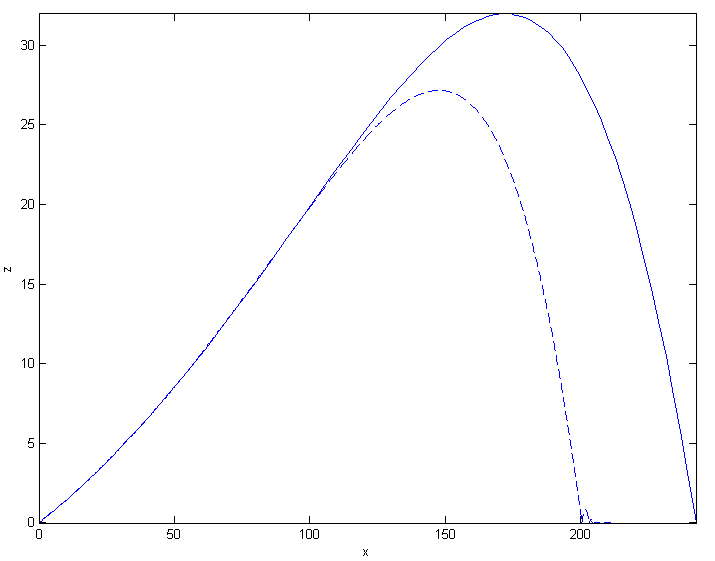
\includegraphics[scale=0.8]{../images/data2-2d.png}
\caption[Second data set using the modified Morrison form.]{Here the dashed line is the second data
set and the solid line is the model using the modified Morrison form.}
\label{data2-2d}
\end{figure}

\section{Parametrising $c_{D}$ and $c_{L}$ by Non Dimensional Variables}

We now attempted a different approach: following the idea of \citet{Lieberman2001} we attempted to
use the data from The R\&A to estimate parameters in functions of dimensionless groupings for $c_D$
and $c_L$. 

\citet{Lieberman2001} give a number of forms for $c_D$ and $c_L$. We will use the first form given in
the patent, that is
\begin{subequations}
\begin{align}
c_D &= \bar{A} + \bar{B} Sr^2 + \bar{C} Re + \bar{D} Sr \\
\shortintertext{and}
c_L &= \hat{A} + \hat{B} Sr + \hat{C} Re^{-2} + \hat{D} Sr^2
\end{align}
\end{subequations}
where $Re$ is the Reynolds number as before, and $Sr$ is the spin ratio, defined as
\begin{equation}
Sr = \frac{|\vec{\omega}|D}{v} .
\end{equation}
The spin ratio another possible dimensionless grouping, which emerges when performing the same analysis
as section \ref{sec:drag} but with $\omega$ and $\theta$ as part of the analysis. $D$ is the diameter
of the golf ball.

The coefficients $\bar{A}, \bar{B}, \bar{C}, \bar{D}, \hat{A}, \hat{B}, \hat{C}, \hat{D}$ are to be
determined using the data. In order to do this, we use a non linear least squares method (see appendix 
\ref{ls}) to fit the parameters within the model to the data set at hand.

In order to solve the problem we must specify an initial guess for the coefficients, before allowing
the least squares algorithm to refine the parameters. The values for the guesses were found by 
simply hand optimizing the functions based on typical speeds and spins for golf balls, changing the
coefficients until the values of $c_D$ and $c_L$ became fairly close to the values we expect them to
take from experiments.

For $c_D$ we take
\[
\bar{A} = \bar{B} = \bar{C} = \bar{D} = 6 \times 10^{-6}
\]
and for $c_L$ we take
\[
\hat{A} = \hat{B} = \hat{C} = \hat{D} = 0.5
\]
as the initial guesses.

Running these against the data provided by The R\&A provides mixed results. For some trajectories, 
the fit is almost perfect in all three dimensions as we see in Figure~\ref{ls-data2-1-2d} and 
Figure~\ref{ls-data2-1-3d}. However,
when using the same ball with different initial conditions we sometimes obtain worse fits, which do not match
as well as the previous data set, for example Figure~\ref{ls-data2-3-2d}. For some of the data sets
the least squares algorithm with the guesses as above cannot fit the data at all, as the new values 
of the parameters estimated render the equations of motion impossible to integrate using the standard routines within
MATLAB and the guesses must be changed to proceed with this data set. This implies that estimating $c_D$
and $c_L$ in this way
is incredibly sensitive to the choice of initial conditions and can only have limited utility if
a person is required to manually change the guesses to make the model work.

\begin{figure}
\centering
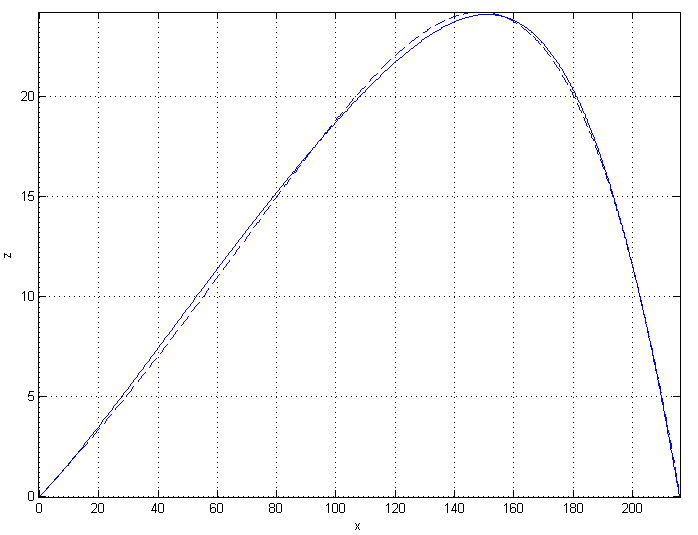
\includegraphics[scale=0.7]{../images/ls-data2-1-2d.png}
\caption[Least squares using the Re and Sr form on data]{Here we plot the least squares fit using
the $c_D$ and $c_L$ from \citet{Lieberman2001} in solid line against the data set it was fitted to
in dashed line. The parameter values for this trajectory are given in Table~\ref{ls-table} in Data set 1.}
\label{ls-data2-1-2d}
\end{figure}

\begin{figure}
\centering
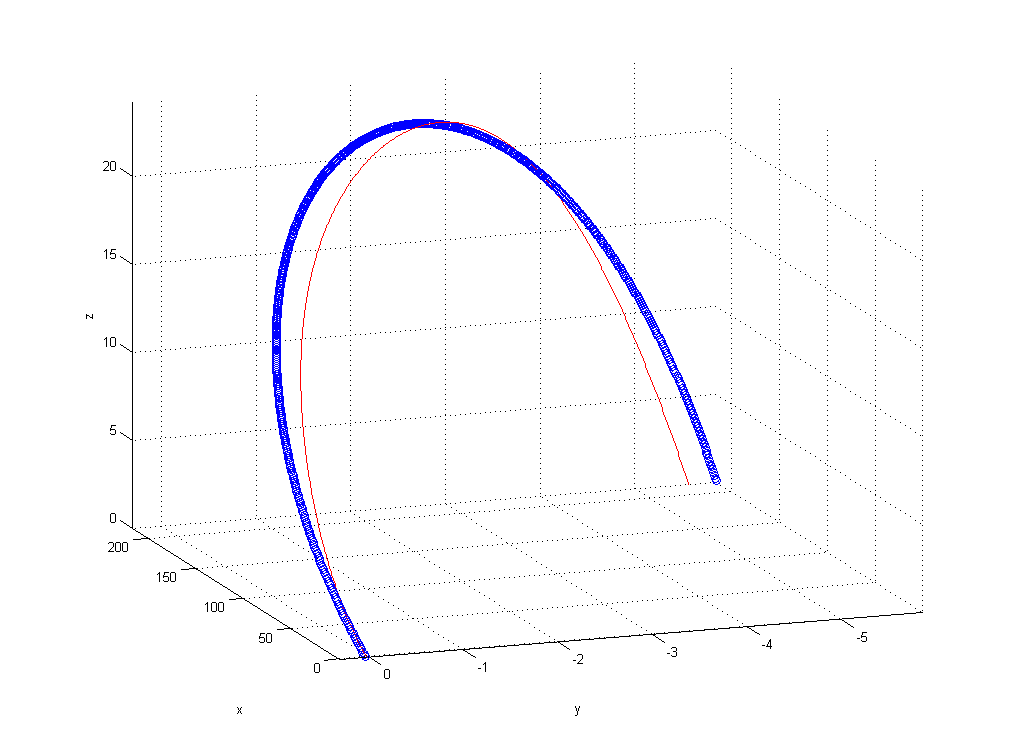
\includegraphics[scale=0.55]{../images/ls-data2-1-3d.png}
\caption[Least squares using the Re and Sr form on data in 3D]{Here we plot the data and trajectory from
Figure~\ref{ls-data2-1-2d} in 3D. Note how close the red model curve has almost identical carry and shape to the thick blue data points.}
\label{ls-data2-1-3d}
\end{figure}

Additionally, when comparing the values of $\bar{A}, \bar{B}, \bar{C}, \bar{D}, \hat{A}, \hat{B}, \hat{C}, \hat{D}$
between data sets taken with the same golf ball, we do not see any regularity for the resultant 
values. The R\&A provided a data set using the same golf ball 4 times with 4 slightly different
initial conditions. If the values of the coefficients $\bar{A}, \bar{B}, \bar{C}, \bar{D}, \hat{A}, \hat{B}, \hat{C}, \hat{D}$
are in some way physical we would expect that between the different measurements the values would stay fairly constant
due to being related to the physics of the ball, rather than just fitting the data and being inconsistent
between different initial conditions. However, as we can see in Table~\ref{ls-table} this is not the case:
the coefficients vary in sign and order of magnitude between each data set with little consistency between
them.

This implies that while it is possible to fit the model data using these forms of $c_D$ and $c_L$
there is no physical data to be gained from using the least squares method here, and it would not
be advisable to use the coefficients from one set of initial conditions to attempt to estimate the
trajectory for another.

\begin{figure}
\centering
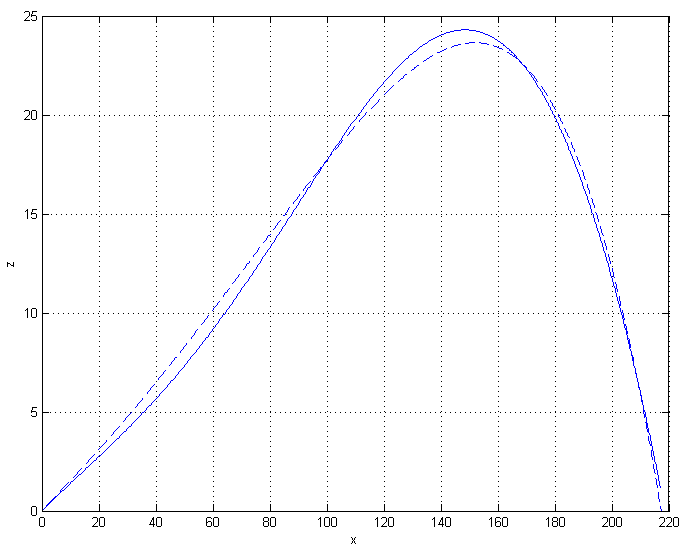
\includegraphics[scale=0.6]{../images/ls-data2-3-2d.png}
\caption[Trajectory which least squares struggles to fit]{Attempting to fit the $c_D$ and $c_L$ from
\citet{Lieberman2001} works slightly less well for this trajectory than for Figure~\ref{ls-data2-1-2d}.
The parameter values for this trajectory are given in Table~\ref{ls-table} in Data set 3.}
\label{ls-data2-3-2d}
\end{figure}

\begin{table}
\footnotesize
\centering
\begin{tabular}{c| c c c c c c c c}
Data set & $\bar{A}$ & $\bar{B}$ & $\bar{C}$ & $\bar{D}$ & $\hat{A}$ & $\hat{B}$ & $\hat{C}$ & $\hat{D}$ \\
\hline
1 & 0.2063 & 0.2211 & -19.5001 & 0.0365 & 4.6830 & 15.9221 & $-1.4540\times10^{-5}$ & -15.9351 \\
2 & 0.0697 & 1.1092 & -14.9529 & -0.8197 & -11.1921 & -24.1217 & $3.9889\times10^{-5}$ & 28.9117 \\
3 & 0.3963 & -1.0174 & 0.4995 & 1.9337 & -6.3150 & -15.9492 & $2.1123\times10^{-5}$ & 17.3877 \\
4 & 0.2229 & 0.0463 & 0.4999 & 0.5278 & -0.7197 & -0.0492 & $3.0765\times10^{-6}$ & 0.4549
\end{tabular} 
\caption[Table of coefficients calculated by the least squares method]{The values of the coefficients 
calculated using least squares for the 4 data sets with the same ball.
}
\label{ls-table}
\end{table}

Since we can fit the modelled trajectories to the data using this method it is useful to try and see
the limitations of this technique. Therefore, we then considered using only a limited portion of 
the data to see if the starting part of the trajectory can determine the full flight of the ball.

To do this, we simply run the same least squares method as before but with a smaller data set, over
say the first 30m of the flight. We then use the predicted coefficients in $c_D$ and $c_L$ to run a
full flight simulation of the ball and compare this to the full data set to ascertain how accurate this
procedure is.

\begin{figure}
\centering
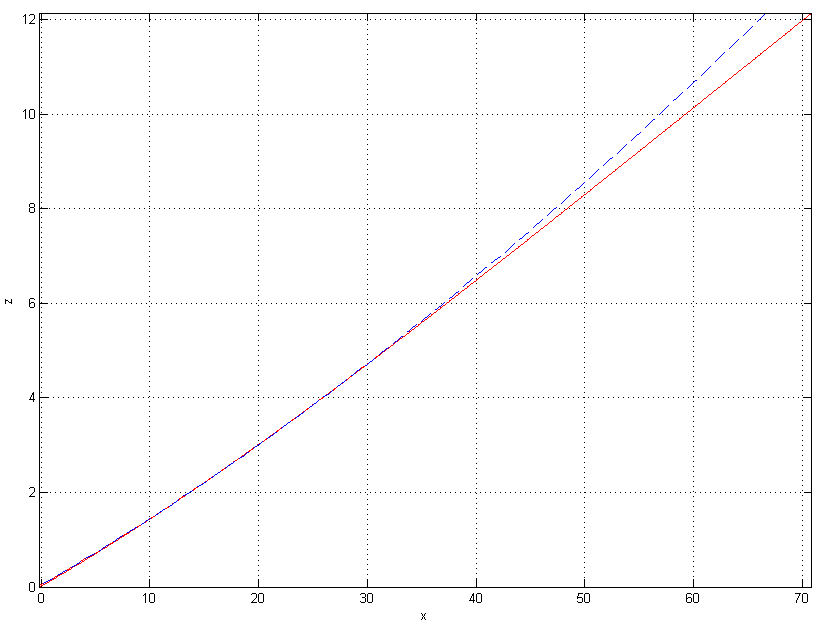
\includegraphics[scale=0.6]{../images/ls-small-start.png}
\caption[Using a smaller section of data in the least squares method]{Here, we plot the data in dashed
line against the least squares fitted model in red solid line. The data used in the least squares fit
is from $x=0$ to $x=30$ and we can see that in this portion the model and the data align perfectly. After
this the model and data begin to deviate slightly.}
\label{ls-small-start}
\end{figure}

\begin{figure}
\centering
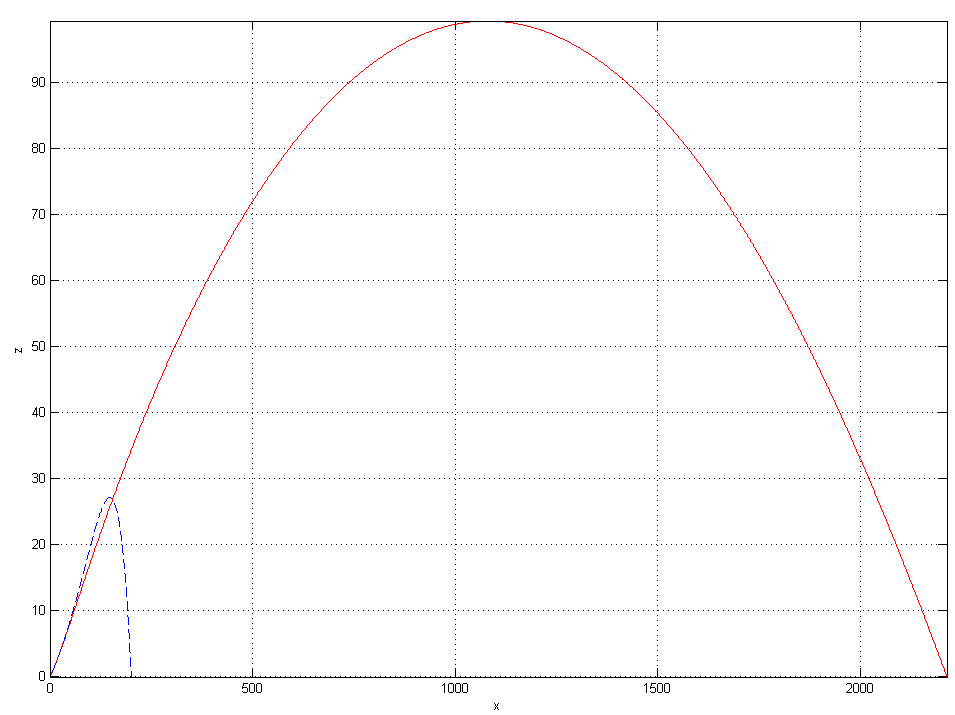
\includegraphics[scale=0.5]{../images/ls-small-full.png}
\caption[Using the parameters from the small least squares run in the full model]{Here we run the model
to the end of the trajectory using the parameters found within Figure~\ref{ls-small-start} using least
squares. The values are wildly inaccurate in both height and carry of the ball.}
\label{ls-small-full}
\end{figure}

For the initial portion of the data the least squares matching does very well as we can see in Figure~\ref{ls-small-start}, 
matching the initial
30m almost perfectly. The residual between the model and the data is very small, approximately 0.0594.
The values of the parameters this model produces are as follows:
\begin{gather*}
\bar{A} = 2.2928, \,\, \bar{B} = -8.8290, \,\, \bar{C} = 0.6996, \,\, \bar{D} = -3.5440, \\
\hat{A} = -4.0220, \,\, \hat{B} = 2.5129, \,\, \hat{C} = 1.2528\times10^{-5}, \,\, \hat{D} = 8.5804
\end{gather*}

On running the model using the values of the parameters estimated above however, it quickly becomes
apparent that the initially good fit is only for the starting portion of the data: the values of the
parameters given massive over estimate the trajectory, with a carry in excess of 2km as we can see in
Figure~\ref{ls-small-full}.

Using the least squares technique allows a good fit for the data to be found when using the whole trajectory,
however estimating the parameters with a small section of the data seems to be beyond the abilities 
of this technique to currently estimate. It may be possible to use more sophisticated numerical techniques
or to set bounds on the parameters to obtain a more realistic set of estimates for the parameters in
$c_D$ and $c_L$ in this form.

% \begin{itemize}
% \item We follow the idea from \citet{Lieberman2001}: form $c_{D}$ and $c_{L}$ from dimensionless
% groupings and use the data to estimate the parameters in this model.
% \item Use least squares to do this. See Appendix for discussion of what an inverse problem is, how
% to use least squares to solve them, and what numerical techniques there are to do this.
% \item Find that doing this is very hard: the problem is likely not well posed and finding a minimum
% is difficult. Would benefit from a more through analysis of the least squares problem but unsure how
% this would be done.
% \item This inverse problem is a good way to move forwards with the problem in the future.
% \end{itemize}

\section{$\tanh$ Matching}

As we have seen in the previous section, using least squares estimates can produce fairly convincing
fits with the experimental data we have been using. However, the physical grounding of these parameters
is unknown: they are simply terms which can be selected from the dimensional analysis of the drag 
and lift functions and form a dimensionless group. There is no experimental evidence that the drag or
lift should take this form.

Thus, instead of attempting to use least squares on a drag form we do not have any physical basis for
we will try a hybrid method between the two ideas: a drag function similar to the modified Morrison
form we have in the first section but parametrised in such a way that we can use the least squares
analysis to find the parameters for a particular ball.

In order to do this we approximate the drag crisis and near linear portions at the subcritical and 
supercritical Reynolds number by a $\tanh$ function of the form
\begin{equation} \label{tanh}
c_{D} = a + b \tanh (-c(Re - d)) .
\end{equation}

The 4 constants $a,b,c,d$ here control the size, shape and position of the drag crisis drop. In particular
\begin{itemize}
\item $a$ controls the placement of the ``middle'' of the drag crisis drop. When $a=0$ the drop passes
through the $Re = 0$ axis.
\item $b$ controls the size of the drop. When $b=1$ and $a=0$ the drop is from $c_D = 1$ to $c_d = -1$.
\item $c$ controls how steep the drop is. As $c$ increases the drop grows asymptotically closer to
a step function like drop.
\item $d$ controls the placement of the drop, effectively shifting the drop to the origin of the
coordinate system.
\end{itemize}

Using the knowledge of how these parameters work we can choose an initial set of $a,b,c,d$ such that
the form of \eqref{tanh} is like that of the modified Morrison drag from section~\ref{morrison}. This
is simple enough that with a few minutes of trial and error the following values may be obtained
\[
a = 0.24, \quad b = 0.17, \quad c = 0.00005, \quad d = 120000 .
\]
These values approximate the modified form of the Morrison drag very well near the drop, as we can see
from Figure~\ref{tanh-init}.

\begin{figure}
\centering
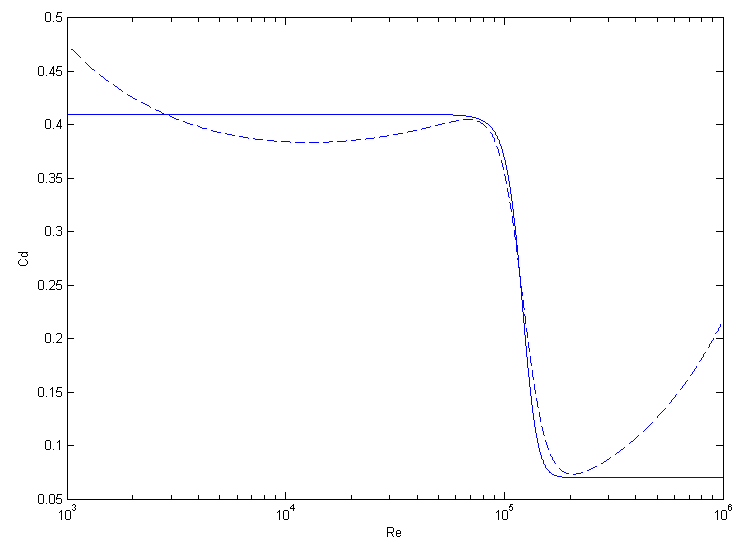
\includegraphics[scale=0.7]{../images/tanh.png}
\caption[The tanh form near the drag crisis]{The $\tanh$ function with $a,b,c,d$ defined as above plotted
in solid line against the modified drag form plotted in dashed line.}
\label{tanh-init}
\end{figure}

Running the model with this initial guess for the coefficients and using data set 1 we obtain a reasonable
approximation to the trajectory as we can see in Figure~\ref{tanh-model}, although not as good as 
we have been able to obtain with other methods.
\begin{figure}
\centering
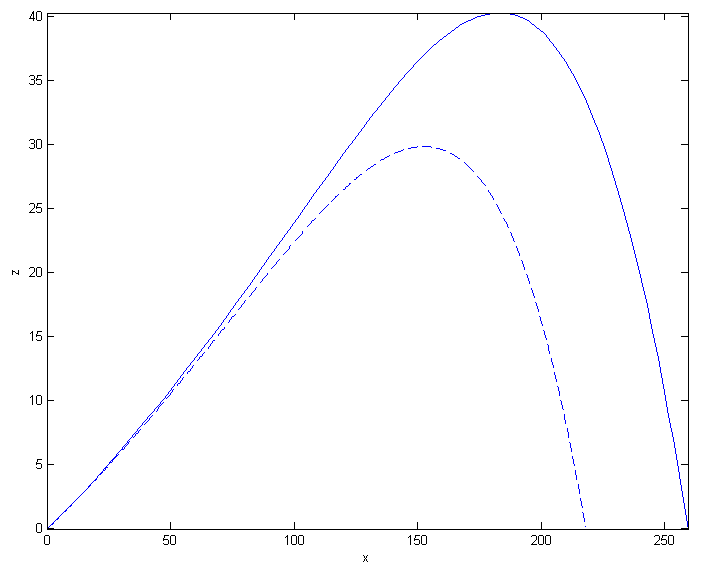
\includegraphics[scale=0.7]{../images/tanh_guess.png}
\caption[Running the initial form of the tanh drag form]{In solid line is the model for this trajectory
using the $\tanh$ form for the drag function. In dashed line is the data for this trajectory.}
\label{tanh-model}
\end{figure}

If we then use least squares algorithm to estimate the parameters unfortunately the solution is not as easy to
obtain than that using the non dimensional variables. Sometimes the solution will be obtained
by the solver, but the height and carry of the ball will be greatly reduced as compared to the data, 
having brought the model into closer agreement with the motion along the $y$ axis at the expense of
the motion along $x$ and $z$. In other cases the solver struggles to find a minimum in the parameter
space at all.

This all implies that as with the previous section there is extreme sensitivity to the choice of 
initial guess for the coefficients in \eqref{tanh}. For example, if we change $d$ in the initial 
guess from $120000$ to $133000$ and leave all the other parameters the same, we find a much closer fit
to the data as we can see in Figure~\ref{tanh_guess2}.
\begin{figure}
\centering
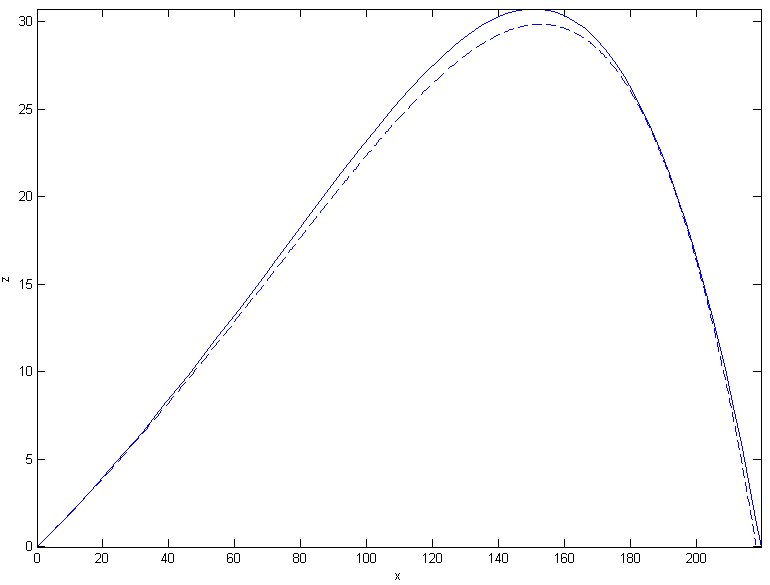
\includegraphics[scale=0.7]{../images/tanh_guess2.png}
\caption[Running the same form as Figure~\ref{tanh-model} with a different value for $d$]{This is the
same trajectory as Figure~\ref{tanh-model} with one of the parameters in \eqref{tanh} modified.}
\label{tanh_guess2}
\end{figure}

There are ways to proceed from here: we
could constrain the problem to be within certain ranges of parameters. However, in doing this we
will inevitably lose some predictive power of the model to detect the physical characteristics of the
golf ball as we desire.
% \begin{itemize}
% \item Take a hybrid approch between the two previous ideas: form a function which ``looks'' similar
% to \citet{Morrison2010} and has the same behaviour, but is parameterised in such a way as to allow
% us to use a least squares solver to estimate parameters.
% \item For the drop, use a $\tanh$ function of the form
% \[
% c_{D} = a + b \tanh (-c(Re - d))
% \]
% where $a,b,c,d$ are constants which we can use least squreas to determine.
% \item Match the $\tanh$ at the top with the $24/Re$ form we know from spheres and past the drop match
% to the weakly linear form we see from the previous work.
% \item Still trying to decide on results for this.
% \end{itemize}
\section{Summary}

Using least squares and more generally inverse problems techniques to estimate the parameters in 
the drag and lift functions for golf balls shows great promise, however we have not been able to 
adequately solve this problem within this project. Continuing this work requires a more thorough
consideration of how to correctly estimate the parameters using inverse problems techniques.

The methods presented in this chapter do show promise however: we can improve the model beyond the
assumptions of \citet{Robinson2013} as we hoped. These open new directions which modelling golf ball
flight can continue into in the future.